\section{Routing in MoE}
\begin{frame}[allowframebreaks]{}
    \LARGE Routing in MoE
\end{frame}

\begin{frame}[allowframebreaks]{Routing in MoE}
    \begin{itemize}
        \item \textbf{Key Concepts:}
        \begin{itemize}
            \item Assign tokens to experts per layer.
            \item Routing can be token-level or batch-level.
            \item Penalize overused experts (using load balancing loss).
            \item Efficient hardware utilization is key.
        \end{itemize}
    \framebreak
        \begin{figure}[h]
            \centering
            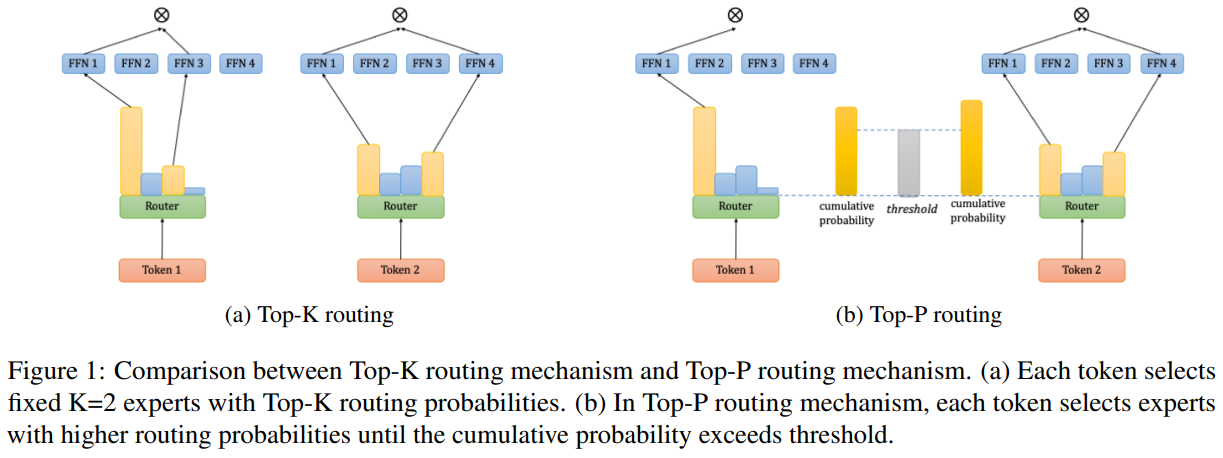
\includegraphics[width=\textwidth,height=0.8\textheight,keepaspectratio]{images/lrm+moe/routing-top-k.png}
            \caption*{Source: \href{https://arxiv.org/abs/2403.07652}{Huandi et al. (2024)}}
        \end{figure}
    \framebreak
        \item \textbf{Example 1: DeepSpeed-MoE}
        \begin{itemize}
            \item Optimizes distributed routing and communication.
            \item Achieves linear scaling to hundreds of experts.
            \item Focuses on efficient data movement across devices.
        \end{itemize}
    \framebreak
        \begin{figure}[h]
            \centering
            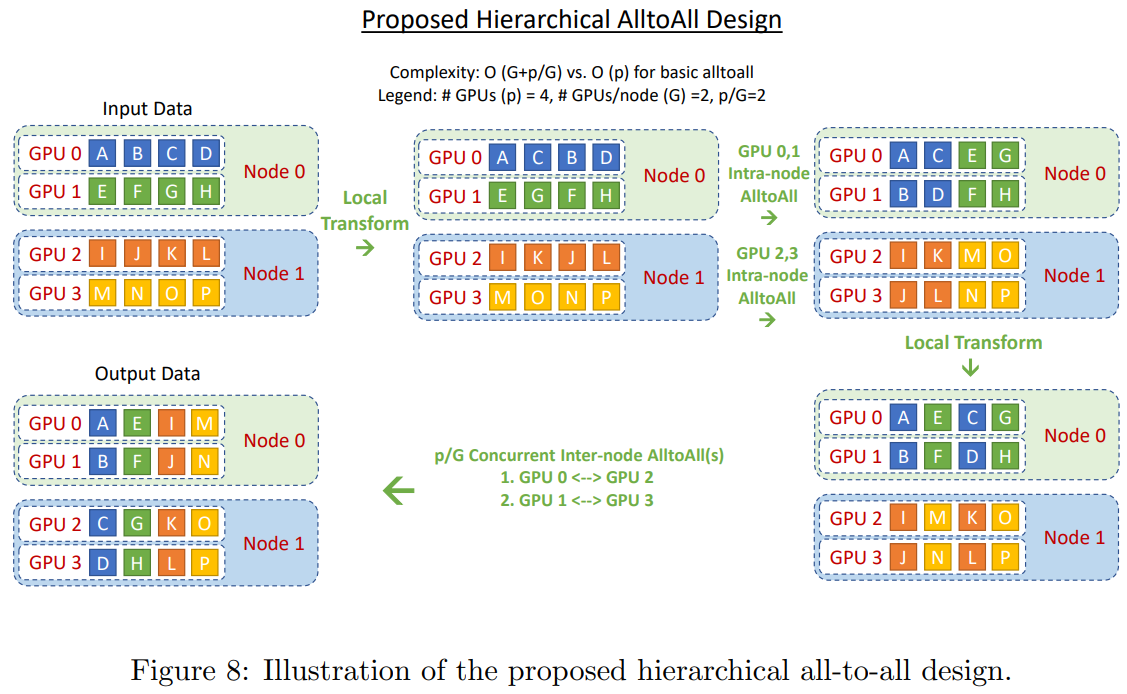
\includegraphics[width=\textwidth,height=0.8\textheight,keepaspectratio]{images/lrm+moe/deepspeed-moe-1.png}
            \caption*{Source: \href{https://arxiv.org/abs/2201.05596}{DeepSpeed-MoE, Rajbhandari et al. (2022)}}
        \end{figure}
    \framebreak
        \begin{figure}[h]
            \centering
            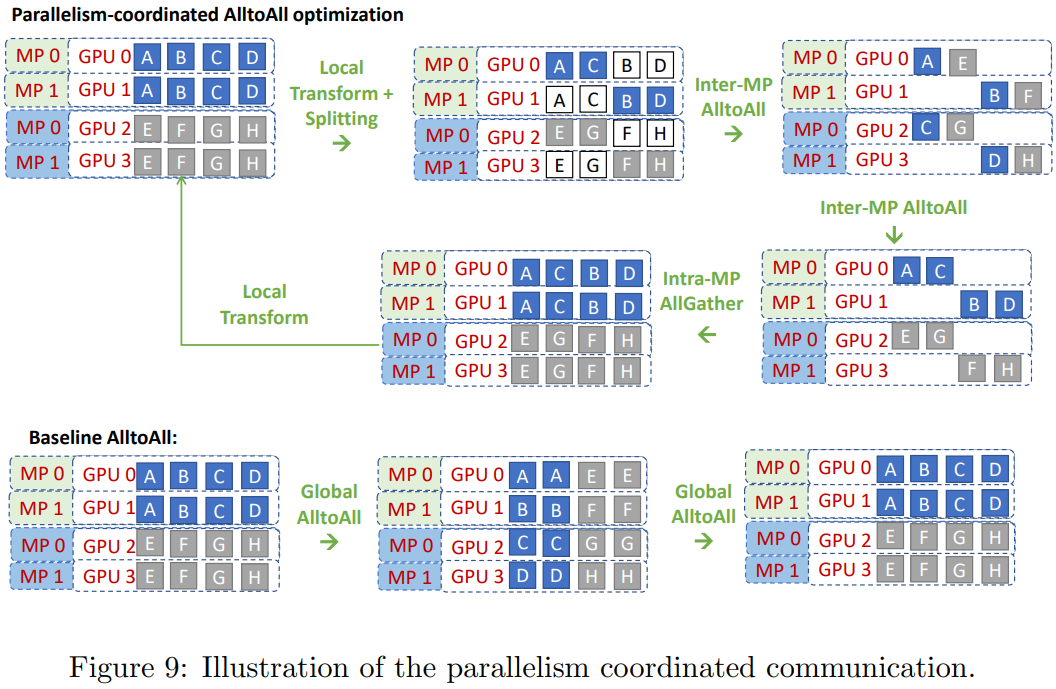
\includegraphics[width=\textwidth,height=0.8\textheight,keepaspectratio]{images/lrm+moe/deepspeed-moe-2.png}
            \caption*{Source: \href{https://arxiv.org/abs/2201.05596}{DeepSpeed-MoE, Rajbhandari et al. (2022)}}
        \end{figure}
    \framebreak
        \item \textbf{Example 2: Tutel by Microsoft}
        \begin{itemize}
            \item Uses custom \textbf{CUDA kernels}.
            \item For highly efficient token routing in MoE.
            \item Reduces overhead and speeds up computation on GPUs.
        \end{itemize}
    \framebreak
        \begin{figure}[h]
            \centering
            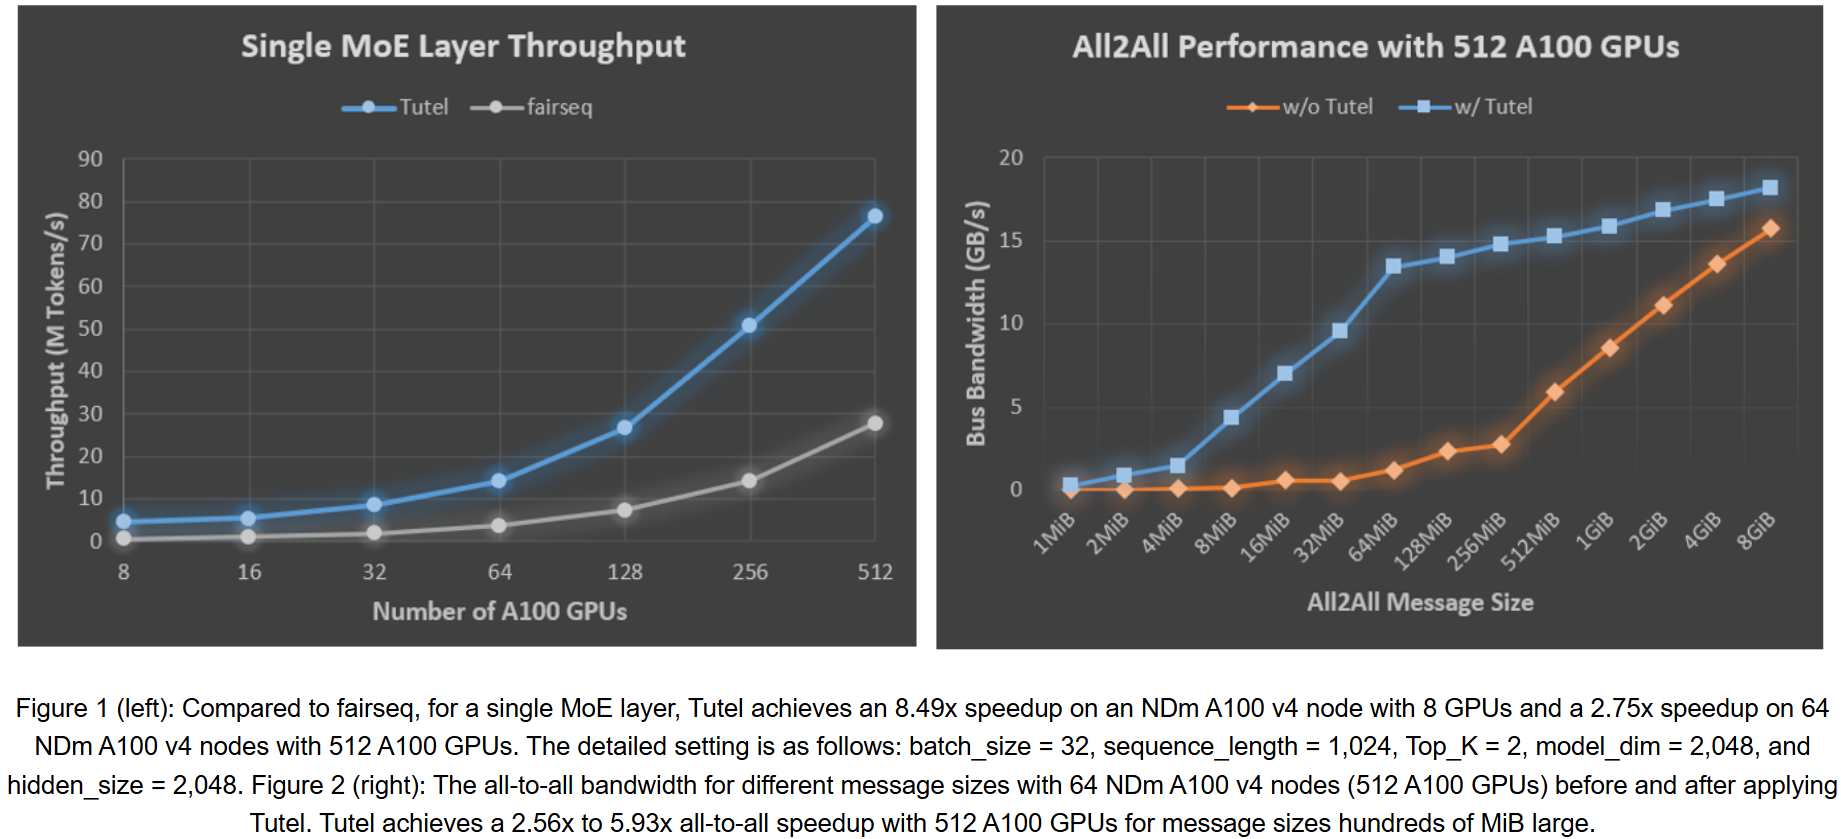
\includegraphics[width=\textwidth,height=0.8\textheight,keepaspectratio]{images/lrm+moe/tutel.png}
            \caption*{Source: \href{https://www.microsoft.com/en-us/research/blog/tutel-an-efficient-mixture-of-experts-implementation-for-large-dnn-model-training/}{Tutel (2021)}}
        \end{figure}
    \end{itemize}
\end{frame}